\chapter{自作モジュールの作成と再利用}
\label{ch:modules}

平均の計算や図の作成を複数の解析で繰り返すときは、その処理を一つのファイルへまとめておくと、使うたびに書き直さずに済む。まず短い平均の関数を保存し、別のファイルから呼び出してみる。その後で、他のプロジェクトへも配れるパッケージの構成と、インストール方法を扱う。

\section{平均の関数を別のファイルから使う}

まず、2 つの測定値の平均を別のファイルから求める。新しい作業用フォルダーを作り、次の内容を \code{signal\_stats.py} という名前で保存する。

\begin{lstlisting}[language=Python, title={signal\_stats.py}]
def mean_signal(values):
    """数値列の算術平均を返す。空列ではValueErrorを出す。"""
    if len(values) == 0:
        raise ValueError("入力列が空です。")
    return sum(values) / len(values)
\end{lstlisting}

同じフォルダーに \code{analyze.py} を作り、次を保存する。

\begin{lstlisting}[language=Python, title={analyze.py}]
from signal_stats import mean_signal

values = [12.4, 15.1]
print(mean_signal(values))
\end{lstlisting}

端末で 2 つのファイルを保存したフォルダーへ移動し、実行する。

\begin{lstlisting}[numbers=none, xleftmargin=2\zw]
$ python analyze.py
13.75
\end{lstlisting}

\code{from signal\_stats import mean\_signal} は、\code{signal\_stats.py} に書いた関数を読み込む命令である。\code{mean\_signal(values)} がその関数を呼び、2 つの測定値の平均を返す。このように読み込んで使う Python ファイルをモジュール\index{もじゅーる@モジュール|textbf}という。

複数のモジュールをディレクトリへまとめ、読み込んで使う単位をパッケージという。同じフォルダーの別のスクリプトからも、この関数を読み込める。他のフォルダーやプロジェクトからも安定して使うには、後で説明するパッケージ\index{ぱっけーじ@パッケージ|textbf}にまとめ、使用する環境へインストールする。次の節からは、その構成を作る理由と手順を扱う。

\section{解析処理を再利用可能な部品へ分ける理由}

処理を役割ごとのモジュールへ分けると、各公開関数に対して独立したテスト、型情報、docstring を用意できる。解析コードで複数の入力やプロジェクトから共有する対象には、次のものがある。

\begin{itemize}
\item データ読み込み関数
\item フィルタ条件やカットの判定関数
\item 図を作成して保存する関数
\item フィット関数やモデル関数
\end{itemize}

同じ処理を複数のスクリプトへコピーすると、それぞれが独立した実装となり、修正内容が一致しなくなる場合がある。自作モジュールから \code{from histfit\_tools import save\_histogram\_with\_fit} のように import すれば、処理のコードを複製せずに一つの実装を共有できる。

\section{引数・設定ファイルとコードを分ける}

第~\ref{sec:command-line-args}~節では、実行時にファイル名などを指定する方法を学んだ。ここでは、繰り返し使う解析条件をどこへ置くかを整理する。

値の配置は、その値が実行ごとに変わるか、複数の実行で共有されるか、プログラムの定義として固定されるかによって決める。すべてをコマンドライン引数にすると、同じ条件を反復する際にも毎回指定が必要となる。

\begin{description}
\item[コマンドライン引数] 実行ごとに変わる値を置く。入力ディレクトリ、出力先、日付範囲、並列数などが典型である。
\item[設定ファイル] プロジェクト単位では固定だが、将来変更し得る値を置く。較正ファイルのパス、検出器 ID、閾値、図の保存形式などが当てはまる。
\item[環境変数] 計算機ごとに異なるデータの置き場所などを渡す。例えば \code{DATA\_ROOT} に保存先を設定する。認証情報を扱う場合はコードや共有ファイルへ直接書かず、利用するサービスの案内に従って管理する。
\item[コード内の定数] 定義として固定したい値や単位変換を書く。\code{NS\_PER\_SECOND} や物理定数のように、意味が仕様として決まっているものを置く。
\end{description}

入力ファイルのパス、出力先、しきい値、作業ディレクトリなどの実行条件は、コードへ直接固定せず、外から指定できるようにする。コードを変更せずに条件を切り替えられれば、同じ処理の再利用と実行条件の再現が容易になる。

\subsection{設定ファイルに解析条件をまとめる}
\index{まじっくなんばー@マジックナンバー|textbf}

実行のたびには変えないものの、解析条件として変更する可能性がある値は、設定ファイルへまとめられる。形式には JSON や TOML などがある。ここでは標準ライブラリだけで扱える JSON の例（\code{config.json}）を示す。

\begin{lstlisting}[numbers=none, xleftmargin=2\zw, title={config.json}]
{
  "calibration_path": "calib/detector_a.csv",
  "coincidence_window_ns": 250,
  "figure_format": "pdf"
}
\end{lstlisting}

この JSON ファイルを Python のスクリプトから読み込む場合のコード例は次のようになる。

\begin{lstlisting}[language=Python]
import json
from pathlib import Path

config = json.loads(Path("config.json").read_text(encoding="utf-8"))
window_ns = config["coincidence_window_ns"]
print(window_ns)
\end{lstlisting}

実行結果は次のようになる。

\begin{lstlisting}[numbers=none, xleftmargin=2\zw]
250
\end{lstlisting}

この \code{250} は、JSON の \code{coincidence\_window\_ns} から読み込んだ値であり、Python コードには直接記述されていない。そのため、コードを変更せずに設定ファイルだけを差し替えられる。Python 3.11 以降では、標準ライブラリの \code{tomllib} で TOML も読み込める。入力パス、出力先、閾値など、実行ごとに変わり得る条件はコードから設定ファイルまたは引数へ分離する。



\code{250} や \code{3600} のような数値が説明や名前なしにコードへ直接記述されていると、その意味や単位を判断しにくい。このような数値はマジックナンバーと呼ばれる。名前の付け方は第~\ref{sec:magic-number}~節で扱った。値が仕様上の定数なら意味と単位を表す名前を付け、実行条件なら引数または設定ファイルへ分離する。

\section{\code{uv} によるパッケージ開発の初期化}

\subsection{作業用プロジェクトの作成}
\index{src layout@src レイアウト|textbf}

本書では、他のコードから \code{import} するライブラリを作るため、\code{uv init --lib} を用いる。次のコマンドによって、ヒストグラム作図用ライブラリの初期構成と依存関係を作成する。

\begin{lstlisting}[numbers=none, xleftmargin=2\zw]
$ mkdir histfit_tools
$ cd histfit_tools
$ uv init --lib
$ uv add numpy matplotlib scipy
$ uv add --dev pytest ruff
$ uv sync
\end{lstlisting}

\code{uv add} で追加した \code{numpy}、\code{matplotlib}、\code{scipy} は、このパッケージの実行時依存関係である。\code{pytest} と \code{ruff} は開発時にだけ使うため、\code{--dev} 付きで追加する。\code{pytest} は公開関数の返り値と例外を検証し、\code{ruff} は \code{uv run ruff check .} によって未使用 import や規則違反を変更記録前に検出する。本章では、公開関数のテストをパッケージ構成の一部として扱う。

この例で作成するディレクトリ構成を次に示す。

\begin{lstlisting}[numbers=none, xleftmargin=2\zw, title={histfit\_tools/ の例}]
.gitignore
.python-version
README.md
pyproject.toml
src/
`-- histfit_tools/
    |-- __init__.py
    |-- py.typed
    |-- models.py
    `-- plotting.py
tests/
`-- test_models.py
\end{lstlisting}

ここで \code{src/} の下にパッケージを置く構成を \code{src} レイアウトという。プロジェクトのルートをカレントディレクトリにしただけでは \code{src/histfit\_tools} を直接 import できないため、インストールされていない作業ツリーを誤って読み込む問題を検出しやすい。\code{py.typed} は、配布したパッケージの型情報を型検査器が利用できることを示す。

\subsection{\code{pyproject.toml} の役割}

パッケージ開発では、\code{pyproject.toml}\index{pyproject.toml@\code{pyproject.toml}|textbf} が中心になる。ここにはパッケージ名、Python バージョン条件、依存関係\index{いそんかんけい@依存関係|textbf}、ビルド方法などを書く。次は各項目の役割を示す簡略例であり、\code{uv init --lib} と \code{uv add} が生成する下限バージョンは実行時の解決結果によって異なる。

\begin{lstlisting}[numbers=none, xleftmargin=2\zw, title={pyproject.toml}]
[project]
name = "histfit_tools"
version = "0.1.0"
description = "Histogram plotting and fitting utilities."
readme = "README.md"
requires-python = ">=3.12"
dependencies = [
  "matplotlib",
  "numpy",
  "scipy",
]

[build-system]
requires = ["uv_build"]
build-backend = "uv_build"

[dependency-groups]
dev = [
  "pytest",
  "ruff",
]
\end{lstlisting}

\code{dependencies} に列挙したライブラリは、このパッケージをインストールするときに実行時依存関係として解決される。実際に生成された \code{pyproject.toml} の \code{[build-system]} には、\code{uv} と互換性のある \code{uv\_build} のバージョン範囲も記録されるため、その範囲を理由なく削除しない。

\code{uv.lock} は、リポジトリ内の開発・検証環境で解決した依存関係を記録する。\code{uv sync} は \code{pyproject.toml} と \code{uv.lock} に基づいて環境を同期する。一方、一般的なビルドフロントエンドがライブラリをインストールするときには、\code{pyproject.toml} のプロジェクト情報と依存関係を参照し、\code{uv.lock} を配布パッケージの依存関係としては用いない。

\section{具体例: ヒストグラムとフィットをまとめたパッケージ}

本節では、1 次元データを受け取り、\code{numpy.histogram} でヒストグラムを作成し、\code{matplotlib} の \code{errorbar} で描画したうえで、必要に応じて \code{scipy.optimize.curve\_fit} のフィット曲線を重ねて保存する関数の実装を扱う。要求仕様は次のとおりである。

\begin{itemize}
\item 入力: データ列と保存先
\item ビン指定: \code{bins} または \code{bin\_width}
\item フィットの切替え: \code{fit=False} ではヒストグラムのみを保存
\item モデル選択: \code{linear}、\code{quadratic}、\code{power\_law}、\code{gaussian}
\item ユーザー定義関数の受付
\item 引数 \code{p0} によるフィット初期値の指定
\end{itemize}

\subsection{型ヒントと結果をまとめるクラス}
\index{くらす@クラス|textbf}\index{かたひんと@型ヒント|textbf}\index{dataclass@\code{dataclass}|textbf}
以降の例には型ヒントを付ける。\code{x: float} は引数の想定型、\code{-> np.ndarray} は返り値の想定型を示すが、記述するだけで実行時の型検査が行われるわけではない。\code{float | None} は浮動小数点数か \code{None}、\code{tuple[float, float]} は二つの浮動小数点数の組を表す。これらの書式を使う例は Python 3.10 以降を前提とする。

クラスは、関連するデータや操作をまとめたオブジェクトの型を定義する。ここでは \code{@dataclass} を使い、保存先、度数、ビン境界、推定値を一つの結果として返す。\code{result.counts} のように属性名で取り出せる。\code{frozen=True} は属性の再代入を禁止するが、属性が参照する NumPy 配列の要素まで変更不能にするものではない。呼び出し可能な関数やオブジェクトを callable といい、\code{Callable[..., np.ndarray]} は引数構成を限定せず NumPy 配列を返す呼び出しを表す型ヒントである。

\subsection{モデル関数の分離}

まず、フィット関数群を \code{models.py} へ切り出す。

\begin{lstlisting}[language=Python, title={src/histfit\_tools/models.py}]
from collections.abc import Callable

import numpy as np

ModelFunc = Callable[..., np.ndarray]


def linear(x: np.ndarray, a: float, b: float) -> np.ndarray:
    """一次関数 y = a x + b を返す。"""
    return a * x + b


def quadratic(x: np.ndarray, a: float, b: float, c: float) -> np.ndarray:
    """二次関数 y = a x^2 + b x + c を返す。"""
    return a * x**2 + b * x + c


def power_law(x: np.ndarray, amplitude: float, alpha: float) -> np.ndarray:
    """べき関数 amplitude * x^alpha を返す。x > 0 を仮定する。"""
    return amplitude * np.power(x, alpha)


def gaussian(
    x: np.ndarray,
    amplitude: float,
    mean: float,
    sigma: float,
    offset: float,
) -> np.ndarray:
    """ガウス関数と定数オフセットを返す。"""
    z = (x - mean) / sigma
    return amplitude * np.exp(-0.5 * z**2) + offset


NAMED_MODELS: dict[str, ModelFunc] = {
    "linear": linear,
    "quadratic": quadratic,
    "power_law": power_law,
    "gaussian": gaussian,
}


def resolve_model(model: str | ModelFunc) -> ModelFunc:
    """名前または callable からフィット関数を返す。"""
    if callable(model):
        return model

    try:
        return NAMED_MODELS[model]
    except KeyError as exc:
        names = ", ".join(sorted(NAMED_MODELS))
        raise ValueError(f"Unknown model: {model}. Choose from {names}.") from exc
\end{lstlisting}

モデル関数を別ファイルへ置くと、作図処理と数学的なモデルが分離される。指数減衰やローレンツ関数を追加する場合も、\code{plotting.py} の変更箇所をモデルの選択と呼び出しに限定できる。

\subsection{\code{pytest} による最小テスト}

\code{tests/test\_models.py} は、\code{models.py} の公開関数が最低限期待通りに振る舞うかを確認するためのファイルである。ここでは、式の値そのもの、ガウス関数の基本的な形、未知のモデル名に対する例外の 3 点だけを確かめておく。

\begin{lstlisting}[language=Python, title={tests/test\_models.py}]
import numpy as np
import pytest

from histfit_tools.models import gaussian, linear, resolve_model


def test_linear_returns_expected_values() -> None:
    x = np.array([0.0, 1.0, 2.0])
    y = linear(x, 2.0, 1.0)
    assert np.allclose(y, [1.0, 3.0, 5.0])


def test_gaussian_has_peak_at_mean() -> None:
    x = np.array([4.0, 5.0, 6.0])
    y = gaussian(x, amplitude=10.0, mean=5.0, sigma=1.0, offset=2.0)
    assert y[1] == pytest.approx(12.0)
    assert y[1] > y[0]
    assert y[0] == pytest.approx(y[2])


def test_resolve_model_rejects_unknown_name() -> None:
    with pytest.raises(ValueError):
        resolve_model("lorentzian")
\end{lstlisting}

最初のテストは一次関数の出力を既知の値と比較する。2 つ目は、ガウス関数が平均値の位置で最大となり、平均値から等距離にある 2 点で同じ値を返すことを検証する。3 つ目は、登録されていないモデル名に対して \code{ValueError} が発生することを検証する。

テストは次のコマンドで実行できる。

\begin{lstlisting}[numbers=none, xleftmargin=2\zw]
$ uv run pytest
$ uv run ruff check .
\end{lstlisting}

\code{pytest} は関数の出力と例外条件を検証し、\code{ruff} は未使用 import や設定した規則への違反を検出する。実行結果と静的検査を分けることで、テストされていない動作と、実行前に検出できる記述上の問題を区別できる。

\subsection{ヒストグラムの作成・保存関数}

ヒストグラムの作成、フィット、保存を担う \code{save\_histogram\_with\_fit} の実装を \code{plotting.py} に置く。

\begin{lstlisting}[language=Python, title={src/histfit\_tools/plotting.py}]
from collections.abc import Sequence
from dataclasses import dataclass
from pathlib import Path

import matplotlib.pyplot as plt
import numpy as np
from numpy.typing import ArrayLike
from scipy.optimize import curve_fit

from .models import ModelFunc, resolve_model


@dataclass(frozen=True)
class HistogramFitResult:
    """保存先、ヒストグラム、フィット結果を保持する。"""

    output_path: Path
    counts: np.ndarray
    bin_edges: np.ndarray
    parameters: np.ndarray | None
    covariance: np.ndarray | None


def _make_bin_edges(
    values: np.ndarray,
    bins: int | Sequence[float] | None,
    bin_width: float | None,
    data_range: tuple[float, float] | None,
) -> np.ndarray:
    if bins is not None and bin_width is not None:
        raise ValueError("Specify either bins or bin_width, not both.")

    if data_range is None:
        low = float(np.min(values))
        high = float(np.max(values))
    else:
        low, high = map(float, data_range)
        if not np.isfinite([low, high]).all() or low >= high:
            raise ValueError("data_range must contain finite low < high.")

    if low == high:
        high = low + 1.0

    if bin_width is not None:
        if not np.isfinite(bin_width) or bin_width <= 0:
            raise ValueError("bin_width must be finite and positive.")
        n_bins = int(np.ceil((high - low) / bin_width))
        return low + np.arange(n_bins + 1) * bin_width

    if bins is None:
        bins = 40

    if isinstance(bins, int):
        if bins <= 0:
            raise ValueError("bins must be positive.")
        return np.linspace(low, high, bins + 1)

    bin_edges = np.asarray(bins, dtype=float)
    if bin_edges.ndim != 1 or bin_edges.size < 2:
        raise ValueError("bins must contain at least two edges.")
    if not np.isfinite(bin_edges).all() or np.any(np.diff(bin_edges) <= 0):
        raise ValueError("bin edges must be finite and strictly increasing.")
    return bin_edges


def save_histogram_with_fit(
    data: ArrayLike,
    output_path: str | Path,
    *,
    bins: int | Sequence[float] | None = None,
    bin_width: float | None = None,
    data_range: tuple[float, float] | None = None,
    fit_model: str | ModelFunc = "gaussian",
    fit: bool = True,
    p0: Sequence[float] | None = None,
    xlabel: str = "x",
    ylabel: str = "Counts",
    title: str | None = None,
) -> HistogramFitResult:
    """ヒストグラムと誤差棒を描き、必要ならフィット線も重ねて保存する。

    Args:
        data: 1 次元データ列。
        output_path: 保存先ファイル名。
        bins: ビン数またはビン境界列。幅も未指定なら 40 ビン。
        bin_width: ビン幅。bins と同時には指定しない。
        data_range: 範囲の下限と上限。幅指定時は上端を切り上げる。
        fit_model: モデル名または自作 callable。
        fit: False ならフィットを実行しない。
        p0: curve_fit へ渡す初期値。
        xlabel: x 軸ラベル。
        ylabel: y 軸ラベル。
        title: 図タイトル。

    Returns:
        保存先、ヒストグラム、フィット結果をまとめたオブジェクト。
    """
    values = np.asarray(data, dtype=float)
    if values.ndim != 1:
        raise ValueError("data must be one-dimensional.")
    if values.size == 0:
        raise ValueError("data must not be empty.")
    if not np.isfinite(values).all():
        raise ValueError("data must contain only finite values.")

    bin_edges = _make_bin_edges(values, bins, bin_width, data_range)
    if fit and not np.allclose(np.diff(bin_edges), np.diff(bin_edges)[0]):
        raise ValueError("Fitting counts requires equal-width bins.")
    counts, bin_edges = np.histogram(values, bins=bin_edges)
    centers = 0.5 * (bin_edges[:-1] + bin_edges[1:])
    errors = np.sqrt(counts)

    fig, ax = plt.subplots()
    try:
        ax.errorbar(centers, counts, yerr=errors, fmt="o", capsize=3, label="data")

        fit_params = None
        fit_cov = None
        if fit:
            model = resolve_model(fit_model)
            sigma = np.where(errors > 0, errors, 1.0)
            fit_params, fit_cov = curve_fit(
                model,
                centers,
                counts,
                p0=p0,
                sigma=sigma,
                absolute_sigma=True,
                maxfev=10000,
            )
            x_fit = np.linspace(bin_edges[0], bin_edges[-1], 400)
            y_fit = model(x_fit, *fit_params)
            ax.plot(x_fit, y_fit, label="fit")

        ax.set_xlabel(xlabel)
        ax.set_ylabel(ylabel)
        if title is not None:
            ax.set_title(title)
        ax.legend()

        output_path = Path(output_path)
        output_path.parent.mkdir(parents=True, exist_ok=True)
        fig.savefig(output_path, dpi=150, bbox_inches="tight")
    finally:
        plt.close(fig)
    return HistogramFitResult(
        output_path=output_path,
        counts=counts,
        bin_edges=bin_edges,
        parameters=fit_params,
        covariance=fit_cov,
    )
\end{lstlisting}

この関数では、ビン境界の決定と作図本体を分けている。こうしておくと、ビン幅指定のロジックだけを単独にテストしやすい。また、\code{fit\_model} が文字列なら既定のモデル群から選び、callable ならそのまま使うので、利用者は既定モデルと自作モデルを同じ引数で扱える。

この関数のフィットは、等幅ビンの中心における度数を最小二乗法で近似する学習用の実装である。不等幅ビンでは幅の違いが度数に入るため、フィットを拒否する。\(\sqrt{N}\) の誤差棒と、空のビンに便宜上与える \(\sigma=1\) は、低計数に対する信頼区間を保証しない。精密な推定にはビン内で積分した期待計数や Poisson 尤度などを検討する。幅を指定すると上端が指定幅に合わせて切り上がるので、実際の範囲は返された \code{bin\_edges} で確認する。

\subsection{\code{\_\_init\_\_.py} による公開インタフェースの整理}
\index{こうかいapi@公開 API|textbf}

他のプログラムから使ってよい関数名や呼び出し方を、公開 API という。パッケージの公開 API に含める関数とクラスは、\code{\_\_init\_\_.py} で再公開する。

\begin{lstlisting}[language=Python, title={src/histfit\_tools/\_\_init\_\_.py}]
"""Histogram plotting and fitting utilities."""

from .models import gaussian, linear, power_law, quadratic
from .plotting import HistogramFitResult, save_histogram_with_fit

__all__ = [
    "gaussian",
    "HistogramFitResult",
    "linear",
    "power_law",
    "quadratic",
    "save_histogram_with_fit",
]
\end{lstlisting}

こうしておけば、利用側は \code{from histfit\_tools import save\_histogram\_with\_fit} と短く書ける。内部ファイル構成を後で整理し直しても、公開 API を保っている限り、利用者側のコードを壊しにくい。

\subsection{使い方の例}

実際にこのパッケージを使うスクリプトは、たとえば次のようになる。

\begin{lstlisting}[language=Python]
from pathlib import Path

import numpy as np

from histfit_tools import save_histogram_with_fit

rng = np.random.default_rng(42)
data = rng.normal(loc=5.0, scale=1.2, size=4000)

fit_result = save_histogram_with_fit(
    data,
    Path("figures/gaussian_fit.png"),
    bins=35,
    fit_model="gaussian",
    p0=[250.0, 5.0, 1.0, 1.0],
    xlabel="signal [mV]",
    title="Gaussian fit example",
)

if fit_result.parameters is not None and fit_result.covariance is not None:
    parameter_errors = np.sqrt(np.diag(fit_result.covariance))
    print(fit_result.parameters)
    print(parameter_errors)

save_histogram_with_fit(
    data,
    Path("figures/hist_only.png"),
    bin_width=0.2,
    fit=False,
    xlabel="signal [mV]",
)
\end{lstlisting}

1 つ目はガウス関数でフィットし、2 つ目は \code{fit=False} としてヒストグラムだけを保存している。ビン数指定とビン幅指定の両方が動くことも、この 2 例で確認できる。

1 つ目の呼び出しで保存される図の例を図~\ref{fig:histfit-module-example} に示す。ヒストグラムは入力した 4000 個の信号値を表し、曲線はビンごとの度数へ当てはめたガウス関数である。この入力は平均 5.0 mV、標準偏差 1.2 mV の正規分布から生成している。返り値の \code{parameters} と \code{covariance} を調べれば、推定した中心と幅、および各パラメータの標準誤差を生成条件と比較できる。図の保存だけでなく、既知の入力に対して推定結果が妥当かどうかも検証する。

\begin{figure}[H]
\centering
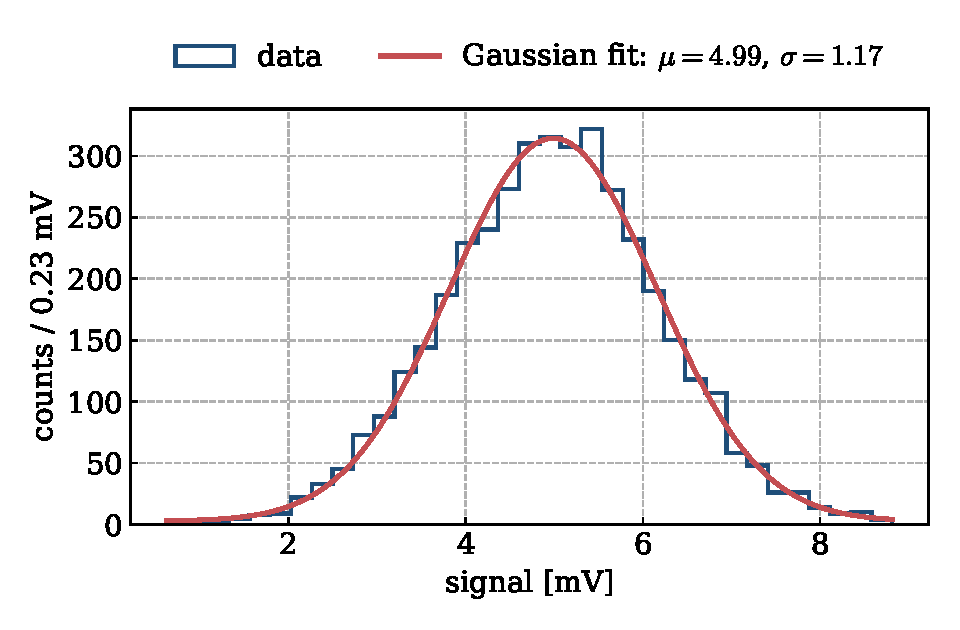
\includegraphics[width=0.72\linewidth]{histfit_module_example.pdf}
\caption{\code{save\_histogram\_with\_fit()} の出力例。ヒストグラムは乱数シード 42 で生成した 4000 個の信号値、実線はガウス関数によるフィットを表す。}
\label{fig:histfit-module-example}
\end{figure}

\code{fit\_model} には、あらかじめ登録した名前だけでなく、同じ呼び出し規約を持つ自作関数も渡せる。指数分布から生成したデータのヒストグラムへ、指数減衰関数を当てはめる例を次に示す。

\begin{lstlisting}[language=Python]
import numpy as np

from histfit_tools import save_histogram_with_fit


def exponential_decay(
    x: np.ndarray,
    amplitude: float,
    tau: float,
    offset: float,
) -> np.ndarray:
    return amplitude * np.exp(-x / tau) + offset


rng = np.random.default_rng(42)
decay_data = rng.exponential(scale=3.0, size=4000)

save_histogram_with_fit(
    decay_data,
    "figures/custom_fit.png",
    bin_width=0.25,
    data_range=(0.0, 15.0),
    fit_model=exponential_decay,
    p0=[300.0, 3.0, 0.0],
)
\end{lstlisting}

\code{fit\_model} は、登録済みのモデル名に加えて、同じ呼び出し規約を持つ callable を受け取る。これにより、パッケージ本体を変更せずに利用者定義のモデルを渡せる。

\section{docstring、型ヒント、README}

自作モジュールには、入力、返り値、例外条件、導入方法を記述する必要がある。関数単位の情報は docstring と型ヒント、パッケージ全体の情報は README が担う。

\subsection{docstring と型ヒント}

docstring\index{docstring@docstring|textbf} には、引数の意味と既定値、返り値、例外条件を記述する。\code{help()} と、docstring 表示に対応したエディタの補完機能は、この情報を参照する。

\code{save\_histogram\_with\_fit} には、\code{data: ArrayLike}、\code{output\_path: str | Path}、\code{fit: bool = True} のような型ヒント\index{かたひんと@型ヒント|textbf}が付いている。VS Code などのエディタでは、関数名にカーソルを合わせたときや補完候補を開いたときに、これらの型ヒントと docstring の先頭が表示されることが多い。したがって、docstring は文書であると同時に、コーディング中に参照できる説明でもある。

docstring の第 1 行には、関数の役割を一文で記述する。たとえば「ヒストグラムと誤差棒を描き、必要ならフィット線も重ねて保存する。」と書き、その後に引数、返り値、例外条件を続ける。

\subsection{README に書くべきこと}

\code{README.md} には、パッケージ全体の目的と導入方法を記述する。この例では次の 4 点を含める。

\begin{itemize}
\item このパッケージが何をするか
\item どうインストールするか
\item 最小の使用例
\item 主要な依存関係
\end{itemize}

たとえば最小限の README は次のようになる。

\begin{lstlisting}[numbers=none, xleftmargin=2\zw, title={README.md}]
# histfit_tools

Histogram plotting and fitting utilities for analysis scripts.

## Installation

```bash
uv venv
uv pip install .
```

## Example

```python
from histfit_tools import save_histogram_with_fit

result = save_histogram_with_fit([1, 2, 2, 3], "example.pdf", bins=3, fit=False)
print(result.counts)
```

## Requirements

Python >= 3.11; NumPy, Matplotlib, SciPy.
Dependencies are installed from pyproject.toml.
\end{lstlisting}

README はパッケージ全体の目的、導入方法、最小使用例を示し、docstring は関数の引数、返り値、例外条件を示す。両者の対象範囲を分け、同じ情報を重複して保守しない。

\section{\code{uv pip} による通常インストールと editable install}

\subsection{通常インストール}

現在のプロジェクト用仮想環境へパッケージを通常インストールするには、パッケージのルートディレクトリで \code{uv pip install .}\index{pip@\code{pip}!install@\code{install}|textbf} を実行する。\code{uv pip} は pip 互換のインターフェースであり、仮想環境内に \code{pip} コマンドがインストールされていない場合にも利用できる。

\begin{lstlisting}[numbers=none, xleftmargin=2\zw]
$ uv pip install .
\end{lstlisting}

これは現在のソースからビルドしたパッケージを環境へインストールする操作である。後から \code{src/histfit\_tools/plotting.py} を編集しても、その変更はインストール済みのパッケージへ自動では反映されない。変更後に \code{uv pip install .} を再実行する。

\subsection{editable install}
\index{editable install@editable install|textbf}

開発中は、\code{uv pip install -e .}\index{pip@\code{pip}!install -e@\code{install -e}|textbf} による editable install を利用できる。

\begin{lstlisting}[numbers=none, xleftmargin=2\zw]
$ uv pip install -e .
\end{lstlisting}

\code{-e} は editable の略であり、インストール先から手元のソースディレクトリを参照できる形でパッケージを登録する。したがって、Python ソースの変更を再インストールせずに import 側へ反映できる。関数定義や docstring を反復して変更する開発環境で用いる。

ただし、editable install が自動的に反映する範囲は、ビルドバックエンドと変更内容に依存する。\code{pyproject.toml} の依存関係を変更した場合や、後述する pybind11 のような C++ 拡張を編集した場合には、環境の同期、再インストール、再ビルドが必要になる。

\subsection{インストール確認}

インストール後は、その仮想環境の Python を直接起動して読み込み元を確認する。\code{uv run} は環境を再同期してプロジェクトを editable install へ戻す場合があるため、通常インストールの確認にはここでは使わない。読み込み済みモジュールはプロセス内に保持されるので、変更後の確認には新しい Python プロセスを使う。

\begin{lstlisting}[numbers=none, xleftmargin=2\zw]
$ .venv/bin/python -c "import histfit_tools; print(histfit_tools.__file__)"
\end{lstlisting}

この import テストは、パッケージ名と公開関数を解決できることを確認する。依存関係、計算、ファイル出力を含む動作は、既知の小規模入力で関数を実行し、返り値と保存ファイルを検証する統合テストで確認する。

\section{Git リポジトリによるパッケージの共有}

研究室内や共同研究で共有する場合は、Git リポジトリによってソース、テスト、設定の変更履歴を管理できる。\code{uv init --lib} は、外側に既存の Git リポジトリがなく、\code{--vcs none} も指定していなければ、初期化対象に \code{.git/} を作る。

GitHub\index{github@GitHub|textbf} で共有する場合は、GitHub の Web 画面でコミットを持たない空のリポジトリを作る。リポジトリ名と公開範囲を指定し、手元にある README と \code{.gitignore} は GitHub 側で重複して作成しない。

空のリモートリポジトリを作成した後、記録対象を確認して次のコマンドを実行する。

\begin{lstlisting}[numbers=none, xleftmargin=2\zw]
$ git add pyproject.toml uv.lock README.md src tests .python-version .gitignore
$ git commit -m "Create histfit_tools package"
$ git branch -M main
$ git remote add origin git@github.com:username/histfit_tools.git
$ git push -u origin main
\end{lstlisting}

\code{uv init --vcs none} のように Git 初期化を明示的に無効化して始めた場合には、最初に \code{git init} が必要になる。

\code{.venv/} や \code{\_\_pycache\_\_/} を追跡対象から除外する規則は、\code{.gitignore} に記述する。Git の状態確認、ステージング、コミット、リモート接続は付録~\ref{app:git} で扱う。

GitHub などに置いたリポジトリを別環境から直接インストールするコマンドは、次のとおりである。

\begin{lstlisting}[numbers=none, xleftmargin=2\zw]
$ uv pip install "git+ssh://git@github.com/username/histfit_tools.git"
\end{lstlisting}

タグやコミットを固定したいなら、URL の末尾に \code{@v0.1.0} や \code{@9f3c1a2} を付ける。

\begin{lstlisting}[numbers=none, xleftmargin=2\zw]
$ uv pip install "git+ssh://git@github.com/username/histfit_tools.git@v0.1.0"
\end{lstlisting}

タグまたはコミットハッシュを URL に含めると、後日の再インストールでも同じリビジョンを指定できる。研究ノートには、インストールに用いた URL とリビジョンを記録する。

\section{実行時依存関係と開発用依存関係}

依存関係については、利用者に必要な実行時依存関係と、開発者だけが使う開発用依存関係を区別する。開発・検証環境の再現にはロックファイルを使う。

\begin{description}
\item[実行時依存関係] パッケージを import して使うだけで必要なもの。今回なら \code{numpy}、\code{matplotlib}、\code{scipy} がこれに当たる。
\item[開発用依存関係] テスト、整形、静的解析にだけ必要なもの。今回なら \code{pytest} や \code{ruff} がこれに当たる。
\item[ローカル環境の固定] 開発者どうしで完全に同じ環境を再現したいときの情報。これは \code{uv.lock} が担う。
\end{description}

ライブラリの \code{dependencies} には、実装とテストによって確認した互換範囲を記述する。根拠なく \code{numpy==2.0.0} のような完全固定を行うと、利用者側の他の依存関係と両立しない場合がある。下限だけを検証した場合は \code{numpy>=2.0} のように記述し、非互換の上限が判明している場合はその上限も記述する。リポジトリ内の開発・検証環境は \code{uv.lock} で再現する。

開発中には、テストや説明文の作成に使う道具も必要になる。これらをすべて実行時依存関係へ含めると、利用者のインストール量と依存関係の衝突リスクが増す。公開 API と実行時依存関係は必要最小限に保ち、開発用の道具は開発用依存関係へ分ける。

\section{章末課題：平均を求めるパッケージを作る}

\begin{enumerate}
\item \begin{minipage}[t]{\linewidth}
\textbf{パッケージを準備する。}
\code{uv init --lib signal\_tools} で作成し、\code{pyproject.toml} と \code{src/signal\_tools/} を確認せよ。ファイル構成を図にし、設定ファイルとコードの役割を説明せよ。
\end{minipage}

\item \begin{minipage}[t]{\linewidth}
\textbf{平均の関数とテストを作る。}
\code{statistics.py} に \code{mean\_signal(values)} を作り、\code{from signal\_tools import mean\_signal} で使えるようにせよ。\code{[1.0, 2.0, 3.0]} では 2.0、空の入力では \code{ValueError} となる 2 件のテストを書く。\code{uv add --dev pytest ruff}、\code{uv run pytest} を実行し、関数と \code{2 passed} の結果を示せ。
\end{minipage}

\item \begin{minipage}[t]{\linewidth}
\textbf{使い方を説明する。}
型ヒントと docstring を付け、\code{help(mean\_signal)} で表示せよ。引数、返り値、空の入力の扱いが分かる使用例を一つ作り、説明文と実行結果を示せ。
\end{minipage}

\item \begin{minipage}[t]{\linewidth}
\textbf{発展：インストール方法を比べる。}
別々の仮想環境へ通常形式と \code{-e} 付きでインストールせよ。実習用に関数の返り値を変更し、再インストール前に反映されるかを表で比較せよ。確認後は正しい関数へ戻し、テストを再実行する。
\end{minipage}

\item \begin{minipage}[t]{\linewidth}
\textbf{共有するファイルを選ぶ。}
NumPy を実行時、pytest と ruff を開発用の依存関係へ追加せよ。\code{.venv/}、\code{\_\_pycache\_\_/}、\code{.pytest\_cache/}、\code{dist/} を \code{.gitignore} へ書く。共有するファイルと生成物を表にし、\code{uv.lock} の扱いも理由とともに説明せよ。
\end{minipage}

\end{enumerate}
